\chapter{Machine Learning as a Modeling Tool} \label{ch:ml}

Machine learning is a branch of artificial intelligence which focuses on using statistical methods to infer relationships, make classifications and predict outcomes. Through increased experience and use of observational data, a learned model can improve its prediction accuracy. There are three types of commonly used methodologies for learning models: 

\begin{enumerate}
    \item \textbf{Supervised learning.} This methodology learns a model based on labeled data. The learning algorithm trains and validates the model against the known ground truth. 
    \item \textbf{Unsupervised learning.} This approach identifies patterns, structures, and features within the data without labels. The algorithm can organize data via clustering, association, autoencoders, and other methods \cite{nvidia}.
    \item \textbf{Reinforcement learning.} An environment and possible discrete states are defined for an agent to transition from one state to another. After the agent takes an action, it gets some amount of reward upon some metric of success, and no reward (or even penalty) upon failure. In doing so, the agent learns the best policy to interact with the environment. 
\end{enumerate}

In this work, a supervised approach is utilized to identify the correlation between inputs and outputs of a black-boxed fiber drawing plant model. After a brief overview of the nomenclature and theory behind neural networks in Section \ref{ch:ml:nn}, Section \ref{ch:ml:rnn} provides the theoretical foundation of this approach, namely a subset of recurrent neural networks called Long Short-Term Memory (LSTM) networks and its variants. 

\section{Preliminaries} \label{ch:ml:nn}

\subsection{Nomenclature and Definitions} \label{ch:ml:nn:def}

The computational paradigm of artificial neural networks (ANNs) draws inspiration from biological neural systems, such as the human brain, to model information flow. A neural network\footnote{Artificial neural networks and neural networks are treated as interchangeable terms.} consists of interconnected elements referred to as \emph{neurons}. A neuron maps a vector of $m$ inputs $\mathbf{x}=\left[x_1, x_2, ..., x_m\right]^T \in \mathbb{R}^{m}$ to a scalar output value $a\in \mathbb{R}$. It is parametrized by a vector of weights $\mathbf{w}=\left[w_1, w_2, ..., w_m\right]^T \in \mathbb{R}^{m}$, in which each element is associated with the input $\mathbf{x}$ at the corresponding index, and the \emph{bias}\footnote{In literature it may be referred to as \emph{offset}, \emph{threshold}, or others.} $w_0$. A neuron is also associated with an \emph{activation function} $f(z): \mathbb{R} \rightarrow \mathbb{R}$, such that\footnote{Some literature writes simply $f\left(\mathbf{w}^T\mathbf{x}\right)$ where  $\mathbf{w}$ and $\mathbf{x}$ has $w_0$ and $x_0$ prefixed into the vector defined above, and $x_0$ is permanently defined as $1$, which yields meaningful calculations in the case of a nonzero bias term \cite{mackay_nn}.}

\begin{equation}
    \label{eqn:activ_fcn}
    a = f(z) = f\left( \sum_{i=1}^n x_i w_i + w_0\right) = f\left(\mathbf{w}^T\mathbf{x} + w_0\right) 
\end{equation}

Some of the most commonly used activation functions are listed in Table \ref{tab:activ_fcns}. The choice of activation function depends specifically on the use case. For instance, LSTM networks, which will be introduced in Section \ref{ch:ml:rnn:lstm}, primarily use sigmoid and hyperbolic tangent activation functions within its structure. Figure \ref{fig:neuron} depicts the basic structure of a single neuron and all operations discussed above. 

\begin{figure}
    \centering
    \includegraphics[width=0.9\textwidth]{figures/neuron.jpeg}
    \caption{Illustration of a single neuron and its operations within \cite{neuron}.}
    \label{fig:neuron}
\end{figure}

\begin{figure}
    \centering
    \resizebox{\textwidth}{!}{
    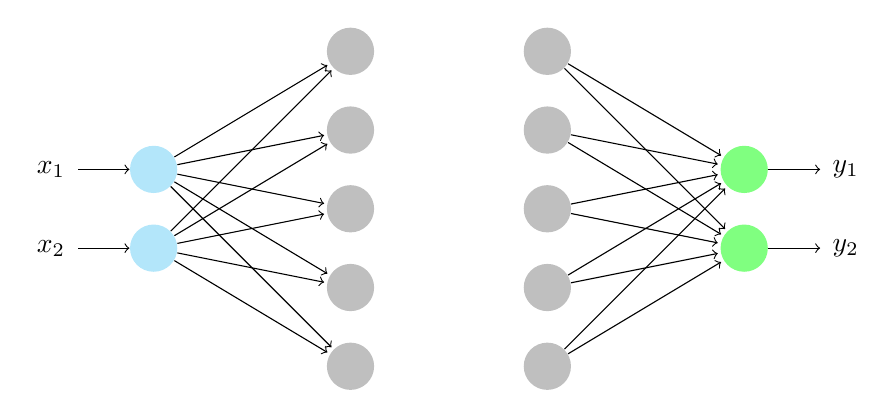
\begin{tikzpicture}
    
    % Input Layer
    \foreach \i in {1,...,2}
    {
    	\node[circle, 
    		minimum size = 6mm,
    		fill=cyan!30] (Input-\i) at (0,-\i) {};
    }
    
    % Hidden Layer
    \foreach \i in {1,...,5}
    {
    	\node[circle, 
    		minimum size = 6mm,
    		fill=gray!50,
    		yshift=3*5 mm
    	] (Hidden1-\i) at (2.5,-\i) {};
    }
    
    \foreach \i in {1,...,5}
    {
    	\node[circle, 
    		minimum size = 6mm,
    		fill=gray!50,
    		yshift=3*5 mm
    	] (Hidden2-\i) at (5,-\i) {};
    }
    
    % Output Layer
    \foreach \i in {1,...,2}
    {
    	\node[circle, 
    		minimum size = 6mm,
    		fill=green!50,
    		yshift=0*5 mm
    	] (Output-\i) at (7.5,-\i) {};
    }
    
    % Connect neurons In-Hidden
    \foreach \i in {1,...,2}
    {
    	\foreach \j in {1,...,5}
    	{
    		\draw[->, shorten >=1pt] (Input-\i) -- (Hidden1-\j);	
    	}
    }
    
    \foreach \m [count=\y] in {missing}
      \node [every neuron/.try, neuron \m/.try ] (hidden-\m) at (3.725,-1.625) {};
    
    % Connect neurons Hidden-Out
    \foreach \i in {1,...,5}
    {
    	\foreach \j in {1,...,2}
    	{
    		\draw[->, shorten >=1pt] (Hidden2-\i) -- (Output-\j);
    	}
    }
    
    % Inputs
    \foreach \i in {1,...,2}
    {            
    	\draw[<-, shorten >=1pt] (Input-\i) -- ++(-1,0)
    		node[left]{$x_{\i}$};
    }
    
    % Outputs
    \foreach \i in {1,...,2}
    {            
    	\draw[->, shorten >=1pt] (Output-\i) -- ++(1,0)
    		node[right]{$y_{\i}$};
    }
    \end{tikzpicture}
    }
    \caption{Illustration of a feedforward neural network. The input, hidden, and output layers are shown in cyan, gray, and green, respectively.}
    \label{fig:nn}
\end{figure}

\begin{table}
    \centering
    \begin{tabular}{c|c|c}
        \textbf{Activation Function} & \textbf{Graph} & \textbf{Usage} \\ \hline \hline
        \makecell{Step function\\ 
        step$(z) =$
            \[\begin{cases} 
                  0 & z < 0 \\
                  1 & z\geq 0 
               \end{cases}
            \]
        }
        & \makecell{\includegraphics[width=4cm]{figures/step.png}} & Binary (0-1) loss \\ \hline
        
        \makecell{Linear Function\\ \\
        $f(z) = z$
        }
        & \makecell{\includegraphics[width=3cm]{figures/linear.png}} & Passthrough \\ \hline
        
        \makecell{Sigmoid/Logistic function\\ \\
        $\sigma(z) = \dfrac{1}{1+e^{-z}}$
        }
        & \makecell{\includegraphics[width=4cm]{figures/sigmoid.png}} & Regression \\ \hline
        
        \makecell{Hyperbolic Tangent (tanh)\\ \\
        $\tanh(z) = \dfrac{e^z-e^{-z}}{e^z+e^{-z}}$
        }
        & \makecell{\includegraphics[width=4cm]{figures/tanh.png}} & Normalizing data \\ \hline
        
        \makecell{\\Softmax function\\ \\
        $\text{softmax}(\mathbf{z}) = \dfrac{\exp(\mathbf{z})}{\sum_{j} \exp(z_j)}$\\ \\
        }
        & \makecell{N/A} & \makecell{Multi-class \\ classification} \\ \hline
        
        \makecell{\\Rectified Linear Unit (ReLU)\\ \\
        ReLU$(z) = $
            \[\begin{cases} 
                  0 & z < 0 \\
                  z & z\geq 0 
               \end{cases}
            \] = \max(0,z) \\ \\
        }
        & \makecell{\includegraphics[width=4cm]{figures/ReLU.png}} & CNNs \\ \hline
        
        \makecell{Leaky ReLU\\ \\
        LReLU$(z) = $
            \[\begin{cases} 
                  \alpha z & z < 0 \\
                  z & z\geq 0 
               \end{cases}
            \], $\alpha > 0$
        }
        & \makecell{\includegraphics[width=4cm]{figures/leaky_relu.png}} & CNNs \\ \hline
        
    \end{tabular}
    \caption{A table of common activation functions, their equations, graphs, and usages\cite{6036}.}
    \label{tab:activ_fcns}
\end{table}

Figure \ref{fig:nn} illustrates the basic anatomy of a \emph{feed-forward neural network}, rightfully named so since its information only flows in the forward direction. Each vertical stack of neurons is called a \emph{layer}. The first layer is called the \emph{input layer}; the layer at which the outputs are generated is called the \emph{output layer}. All intermediate layers in between are called \emph{hidden layers}, and they often represent intermediate or internal representations of the information. For a layer with $n$ units (therefore $n$ outputs) and $m$ inputs, we can denote the weight matrix $\mathbf{W}$ of this particular layer as an $m\times n$ matrix\footnote{Aligning with conventional standards, uppercase bold letters indicate matrices and lowercase bold letters indicate vectors.}, and the output of this layer is expressed as

\begin{equation}
    \label{eqn:layer}
    \mathbf{a} = f(\mathbf{z}) = f\left( \sum_{i=1}^n \mathbf{W}^T\mathbf{x} + \mathbf{w}_0\right) 
\end{equation}
where the bias vector $\mathbf{w}_0 \in \mathbb{R}^n$ and layer output $\mathbf{a} \in \mathbb{R}^n$. 

Recently, a machine learning technique known as \emph{deep learning} has been gaining popularity. Deep neural networks are ones with a large amount of hidden layers, potentially as many as 150. Deep learning has been proven to outperform traditional learning algorithms when presented with a large amount of data \cite{andrew_ng}. The increased parameter space in deep neural networks naturally lends itself to more complex problems such as speech recognition, image classification, and natural language processing. 


\subsection{Supervised Training} \label{ch:ml:nn:train}

Neural networks are often utilized in supervised learning to solve a classification or regression problem. Through the training process, the weights within the neural network are learned to minimize the \emph{loss function}\footnote{Also known as the \emph{objective function} or \emph{cost function} in literature.} $J$, which measures how accurate each of the network outputs are to the corresponding label. Loss functions may take many forms; a selected list of the most common cost functions are enumerated in Table \ref{tab:loss_fcns}. 

% MIGHT REMOVE BOTH TABLES 
\begin{table}[]
    \centering
    \resizebox{\textwidth}{!}{
    \begin{tabular}{c|c|c}
         Name & Equation & Usage  \\ \hline
         
         Binary loss & $L(y,\hat{y}) = $
            \[\begin{cases} 
                  0 & y=\hat{y} \\
                  1 & otherwise 
               \end{cases}
            \]
            & Finite domains \\ 
        
        Linear/L1 loss & $L(y,\hat{y}) = |y-\hat{y}|$ & Regression with outliers \\ 
        Squared/L2 loss & $L(y,\hat{y}) = (y-\hat{y})^2$ & Regression \\ 
        Cross-entropy loss & $L(y,\hat{y}) = -\left[y_i\log \hat{y}_i +(1-y_i)\log (1-\hat{y}_i)\right]$ & Classification
        
    \end{tabular}
    }
    \caption{Common loss functions.}
    \label{tab:loss_fcns}
\end{table}

In other words, training of neural networks is an optimization process in which weights are chosen to minimize the cost function. Most commonly, neural networks are trained using variants of \emph{gradient descent} approaches. The derivative of the cost function with respect to the weights $\mathbf{w}$ (also known as the \emph{network gradient}) is calculated by repeatedly applying the chain rule, in a process known as \emph{backpropagation} \cite{rumelhart_backprop}.

% maybe draw a NN, write out all derivatives, and explain back prop??

Once the network gradient is obtained, the weights are adjusted in the direction opposite to the network gradient, the sensitivity of which is parametrized by the \emph{learning rate} $\eta$. Mathematically, a parameter $\theta$ is iterated as follows, 

\begin{equation}
    \label{eqn:lr}
    \theta \leftarrow \theta - \eta \cdot \nabla_\theta J(\theta) 
\end{equation}

\begin{figure}[t!]
    \centering
    \includegraphics[width=\textwidth]{figures/lr.png}
    \caption{Effects of learning rate on loss minimization \cite{dl_patterson}.}
    \label{fig:lr}
\end{figure}

As shown in Figure \ref{fig:lr}, a learning rate too low requires many iterations and impedes the speed of learning, whereas a learning rate too high may overshoot and lead to divergent behaviors that never reach the desired minimum of the optimization landscape. Selecting an appropriate learning rate, which can converge without sacrificing the speed of learning, is more of an experimental exercise than an analytical one. Especially for deep neural networks, choosing a scheduled, adaptive learning rate can greatly accelerate the training process. There are commonly used decaying learning rate schedules such as exponential, linear, or piecewise\cite{dl_patterson}. In addition, algorithms such as Adagrad \cite{duchi_adagrad}, Adam \cite{kingma_adam}, RMSprop \cite{hinton_rmsprop}, and Nesterov Accelerated Gradient \cite{nesterov_nag}, have been widely used in many applications. 

For deep neural networks, the training process involves dividing the dataset into \emph{batches} and iterating over all the training dataset for multiple \emph{epochs}. In each iteration of an epoch, some \emph{batch size} of data are presented to the network, and the network gradient of all weights are computed based on the loss function calculated with said batches of data. The effects of these hyperparameters, such as learning rate, batch size, and number of epochs, are studied extensively with different datasets. \cite{batch_size_dynamics, batch_size} The consensus in literature suggests that large batch sizes are detrimental to the network's ability to generalize, whereas smaller batch sizes and lower learning rates are beneficial only for fine-tuning purposes, although reaching global optima is not guaranteed due to the non-convexity of the landscape. In general, these effects in the training process depends heavily on the model, the specific usage, and the datasets themselves. 

Furthermore, there are other components to training the neural network, among which are parameter regularization techniques, such as dropout and batch normalization \cite{batch_norm}. Many textbooks are written to provide guidelines to effectively process data and train neural networks. \cite{dl_patterson} and \cite{ml_book_chollet}, for example, give a comprehensive treatment on these topics. 

\section{Recurrent Neural Networks}\label{ch:ml:rnn}

\subsection{Theory of RNNs} \label{ch:ml:rnn:theory}

In contrast to feedforward neural networks discussed above, recurrent neural networks \cite{rumelhart_backprop} have internal feedback loops in their structures, as shown in Figure \ref{fig:rnn}. The feedback of information is especially important for maintain internal state(s) when processing sequential data. For this reason, RNNs have received increasing popularity across a variety of disciplines including natural language processing \cite{rnn_nlp}, speech recognition \cite{rnn_speech_recog}, machine translation \cite{rnn_machine_trans}, and many more. 

\begin{figure}[t!]
    \centering
    \includegraphics[width=0.7\textwidth]{figures/rnn.png}
    \caption{Structure of a simple RNN unit, modeled as a state machine.}
    \label{fig:rnn}
\end{figure}

The information flow in RNNs can be modeled as a state machine with state equations shown in Eq. \ref{eqn:rnn}. 
\begin{equation}
    \label{eqn:rnn}
    \begin{split}
        & s_t = f(s_{t-1}, u_t) \\
        & y_t = g(s_t)
    \end{split}
\end{equation}

where $s_t$ represents the state, $u_t$ the input, and $y_t$ the output at time $t$. The state activation function $f(\cdot )$ resides in the hidden layer; it represents the internal dynamics of a recurrent cell and relates the previous state and input to current state. The output activation function $g(\cdot )$ relates the current state to the output. 

The weights within RNNs are trained through an algorithm known as \emph{backpropagation through time} (BPTT), which unfolds a RNN in time and applies backpropagation (discussed in Section \ref{ch:ml:nn:train}) to find the gradient of the network cost with respect to network parameters. 

% MATH FROM https://d2l.ai/chapter_recurrent-neural-networks/bptt.html, PSEUDOCODE FROM BPTT WIKIPEDIA
% keep it brief and concise

Training RNNs, especially deep RNNs, remains a difficult task in the research community. The backpropagation (discussed in Section \ref{ch:ml:nn:train}) and, by extension, the BPTT algorithm (discussed above) suffer from the exponential growth or decay of the propagated network gradient, phenomena referred to as \emph{exploding gradient} and \emph{vanishing gradient}, respectively \cite{gradient}. 
% math behind vanishing / exploding gradient
% In other words, the error gradients are multiplied repeatedly by copies of the same weight matrix... %CHECK ON THIS
For this reason, the exploding and vanishing gradient problem impedes learning of deep neural networks, as weights closer to the beginning of the network cannot be properly updated after several iterations. There are several heuristics in literature developed to mitigate the exploding gradient problem, such as gradient clipping and weight regularization \cite{gradient}. They do, however, introduce additional hyperparameters to be tuned. Overcoming the vanishing gradient problem was proven to be even more difficult \cite{vanish_grad_difficult}. In the following subsection, I will introduce a subset of RNNs, known as Long Short-Term Memory (LSTM) networks, that partially addresses the exploding and vanishing gradient problem and is found to be better suited for time-series system identification.

\subsection{Long Short-Term Memory Networks} \label{ch:ml:rnn:lstm}

Introduced in 1997 by Hochreiter \& Schmidhuber \cite{lstm_hochreiter}, LSTM networks grew in popularity as a robust and trainable RNN model for sequential data. An illustration of a typical LSTM cell is shown in Figure \ref{fig:lstm}. In its architecture, LSTM networks consist of cells with gating mechanisms, with which the network can have "memory" and retain information over multiple timesteps. The information flow through these gates and their associated update rules are described below; in each LSTM cell, there is a

\begin{itemize}
    \item \emph{Forget gate}, which is typically a sigmoid function (refer to Table \ref{tab:activ_fcns}), that decides whether information should be forgotten (if sigmoid output is near 0) or retained (if sigmoid output is near 1). It is applied to the previous hidden state $h_{t-1}$ and produces the \emph{forget vector} $f_t$.
    \begin{equation}
        f_t = \sigma \left(W_f\cdot \left[h_{t-1},x_t\right]+b_f\right)
    \end{equation}
    \item \emph{Input gate}, which decides what new information should be stored in the cell state $C_t$. It is a combination of a sigmoid function that decides which values to update, and a tanh function that creates a vector of new candidate values.
    \begin{equation}
        \begin{split}
            i_t & = \sigma \left(W_i\cdot \left[h_{t-1},x_t\right]+b_i\right) \\
            \Tilde{C}_t & = \tanh\left(W_C\cdot \left[h_{t-1},x_t\right]+b_C\right) \\
            C_t & = f_t\cdot C_{t-1} + i_t \cdot \Tilde{C}_t
        \end{split}
    \end{equation}
    \item \emph{Output gate}, which multiplies the sigmoid-filtered hidden state and the tanh-filtered cell state $C_t$. The output is the next hidden state $h_t$. 
    \begin{equation}
        \begin{split}
            o_t & = \sigma \left(W_o\cdot \left[h_{t-1},x_t\right]+b_o\right) \\
            h_t & = o_t \cdot \tanh(C_t)
        \end{split}
    \end{equation}
    where $W$'s and $b$'s are the weight parameter matrix and bias terms, respectively, associated with each variable.
\end{itemize}

\begin{figure}[b!]
    \centering
    \includegraphics[width=0.6\textwidth]{figures/lstm.png}
    \caption{Illustration of a typical LSTM cell and the operations within \cite{lstm_olah}.}
    \label{fig:lstm}
\end{figure}

Besides the vanilla version of LSTM network discussed above, other variants have also been introduced. One of such variants explored in this work is the \emph{bidirectional LSTM} (biLSTM) network \cite{brnn_schuster}, which examine the data from beginning to end and from end to beginning. With each input flowing in two directions, the network preserves past and future information. Training two LSTM structures allows the learning algorithm to increase the amount of information available and provide more context to the network. This methodology of learning bidirectional dependencies within sequential data has demonstrated success in speech recognition, forecast prediction, and other signal-based machine learning problems  \cite{bilstm_speech, bilstm_speech2, bilstm_pred}. 

Gonzalez and Yu's work \cite{gonzalez} also explored a rectangular array of LSTM networks and achieved improved performance. The rectangular arrays stacked height-wise resulted in a lower root-mean-square error than the ones stacked width-wise. Parts of the experiments with network architectures are inspired by these cited literature and their performance will be evaluated in Chapter \ref{ch:exp}. 

\section{Relation to System Dynamics Modeling} \label{ch:ml:relation}

Evidently, the mathematics behind ANNs is well-developed and understood. In recent years, the rapid advancement in computational power and explosion in volume of enriching data have added incredible momentum for the machine learning community. ANNs have been used in finance \cite{ann_finance}, medicine \cite{ann_med}, and manufacturing \cite{ann_manu} alike. It has also gained popularity in the controls community for system identification purposes. An advantage of fitting the data to an LSTM model is that the nonlinear system representation can be obtained without the full knowledge of the system \cite{wagh}, which makes the black-box modeling approach plausible. An increasing amount of papers \cite{gonzalez, wang} justify this kind of usage by pointing to the \emph{Universal Approximation Theorem} (UAT), presented below.

\begin{theorem} \label{thm:uat}
\textbf{- Universal Approximation Theorem}

Let $I_m$ denote the $m$-dimensional unit hypercube $[0,1]^m$, and $C(I_m)$ denote the space of continuous functions in $I_m$. Let $\varphi(t)$ be a bounded, continuous function, $\alpha_i, b_i \in \mathbb{R}$, and the weights $w_i\in \mathbb{R}^m$. For any continuous function $f\in C(I_m)$ and $\varepsilon>0$, there exists an integer $N$ (namely, the number of neurons in a layer) such that we may define

\begin{equation}
    F(x) = \sum_{i=1}^N \alpha_i \cdot \varphi(w_i^T x + b_i)
\end{equation}

to be an approximate realization of $f$ arbitrarily close, i.e.

\begin{equation}
    |F(x)-f(x)| < \varepsilon, \texttt{    } \forall x\in I_m
\end{equation}

\end{theorem}

The original UAT \cite{cybenko_1989} guaranteed arbitrary approximation accuracy only for feedforward neural networks with one hidden layer and sigmoid-like activation functions. In 1991, Hornik et al. expanded this notion to multilayer feedforward networks with any activation functions. \cite{hornik_uat} This is a powerful result — it demonstrates that neural networks are universal approximators that can "learn" any continuous function to arbitrarily close accuracy. 

The UAT, therefore, validates the capability of neural networks to model system dynamics, especially nonlinear dynamics that conventional linearized models often fail to capture. ANN-based models can achieve higher dimension with its number of trainable parameters, given a sufficient amount of training data. For instance, a study from Egorchev et al. \cite{egorchev} demonstrated a successful RNN-based approach in modeling an aircraft's rotational motion, a highly nonlinear dynamical system. RNNs are especially capable of capturing system dynamics because they are characterized by sets of coupled nonlinear differential equations. In fact, one can quickly draw similarities between the general representation of nonlinear system dynamics and that of RNNs. Conventionally, a nonlinear system is modeled with the general form 
\begin{equation}
    \label{eqn:nonlinear_cts}
    \begin{split}
        \Dot{\mathbf{x}}(t) & = f\left(\mathbf{x}(t), \mathbf{u}(t) \right) \\
        \mathbf{y}(t) & = g\left(\mathbf{x}(t)\right)
    \end{split}
\end{equation}
or, in the discrete case, 
\begin{equation}
    \label{eqn:nonlinear_discrete}
    \begin{split}
        \Dot{\mathbf{x}}(k) & = f\left(\mathbf{x}(k-1),...,\mathbf{x}(k-n), \mathbf{u}(k-1),...,\mathbf{u}(k-m) \right) \\
        \mathbf{y}(k) & = g\left(\mathbf{x}(k)\right)
    \end{split}
\end{equation}
where $t \in \mathbb{R}^+$, $k \in \mathbb{Z}^+$, $\mathbf{x}(\cdot)$ is the system state vector, $\mathbf{u}(\cdot)$ the system input, and $\mathbf{y}(\cdot)$ the system output. $f$ and $g$ may be nonlinear mappings \cite{wang}. Comparing the above equations to Eq. \ref{eqn:rnn}, it is evident that RNNs can adequately represent discrete nonlinear systems in general.

It has also been observed that, by the recurrent nature of RNNs, deeper RNNs have the advantage in modeling long-term dependencies within sequences and signals, whereas shallower ones tend to pick up the high-frequency, more immediate correlations \cite{drnn}. However, as mentioned in Section \ref{ch:ml:rnn:theory}, vanishing gradient is a known, prominent problem in training neural networks. As a consequence, long-term memory effects are difficult to train. LSTM networks solve this issue with the presence of its forget gate activations; specifically, its cell state gradients are additive and have no exponential factors involved. Consequently, there exists at least one path with a non-vanishing gradient \cite{arbel_lstm_gradient}. This property justifies the use of LSTM as the network architecture of choice in modeling system dynamics, the results of which will be presented in full detail in Chapter \ref{ch:exp}. 